\chapter*{}

Os Hupd'äh contam muitas histórias sobre pessoas que, andando pela mata, se
encontraram com seres da Gente-Sombra.

Os homens e mulheres-sombra são muito fortes e perigosos. Eles usam várias roupas de cores diferentes para caçar e fazer mal às pessoas hup. Uma dessas roupas tem cor de sombra,
daí o seu nome.

A Gente-Sombra causa doenças e pode matar e comer a carne e o espírito das pessoas humanas. Mas muitos deles são sábios, e conhecem cantos, mitos e benzimentos.

Esta é a história do encontro de um homem hup com um homem-sombra chamado Way Naku.

\openany

\blankpage
\part[Os cantos do homem-sombra]{Os cantos do homem-sombra\\Batɨ´b’ yám pɨnɨ´g}


\chapter*{}

\mbox{}\vspace*{\fill}

No alto de uma árvore de
cucura, um homem-sombra
chamado Way Naku cantava
um \textit{caapivaiá}.

\bigskip

Batɨ̗b’ mah yup, Way Naku
batɨ̗b’ mah yup pö̗h yamah,
pɨ̗g tëganah.

\vspace*{\fill}

\blankpage

\chapter*{}

\mbox{}\vspace*{\fill}

Encantado com a música,
um homem hup aproximou-se, sentou-se ao pé da
árvore e ficou escutando as
canções do homem-sombra. O
homem hup estava sentado,
pescando no igarapé
enquanto ouvia a música.

\bigskip

Pɨ̗~g tëgan tɨh yam mɨ’ mah,
hup tɨh mɨ’ wɨ’ pemeh, tú.
Dë̖h máh hõ̖p käk pemep ɨ~hɨ~h.

\vspace*{\fill}

\begin{figure}
\vspace*{-1.2cm}
\hspace*{-2.2cm}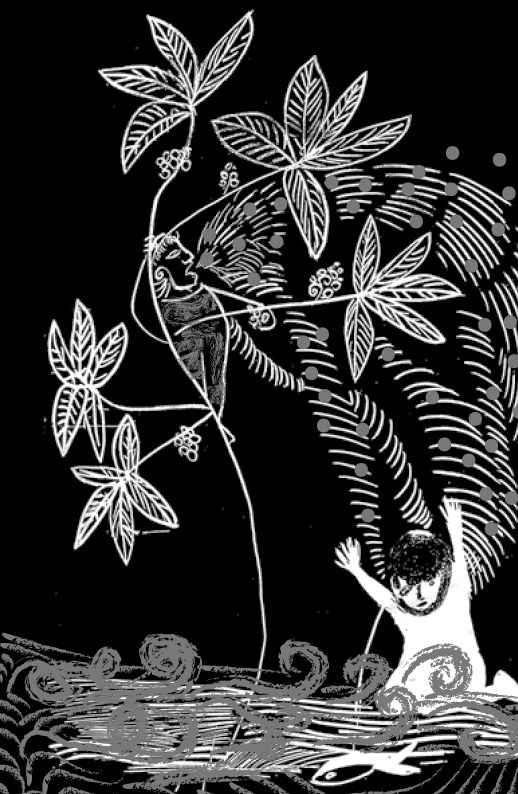
\includegraphics[width=138mm]{./imgs/img2.jpg}
\end{figure}

\chapter*{}

\mbox{}\vspace*{\fill}

Dizem que o Way Naku ficou
cantando e colhendo cucura
por muito tempo. O homem-sombra ia de galho em galho
cantando e pegando os cachos
da fruta. Muitos dos cantos
que nós Hupd’äh cantamos nas
festas foram cantados pelo Way
Naku: o Canto do Cutia, o Canto
Grande, o Canto do Umarí, o
Canto da Gente-Sombra.

\bigskip

Bíg! mah tɨh yamah. Sãp nowot
pid, sãp nowot pid, pɨ̗g tëgët
tɨh noh k’ët kötöh, yamap ihih,
batɨ̗b’ih. Mèt Yam, Yam Pög, Pej
D’áp Yam, Batɨ̗b’ Yam, yám nihu’
mah tíh yamah!

\vspace*{\fill}

\begin{figure}
\vspace*{-1.2cm}
\hspace*{-2.2cm}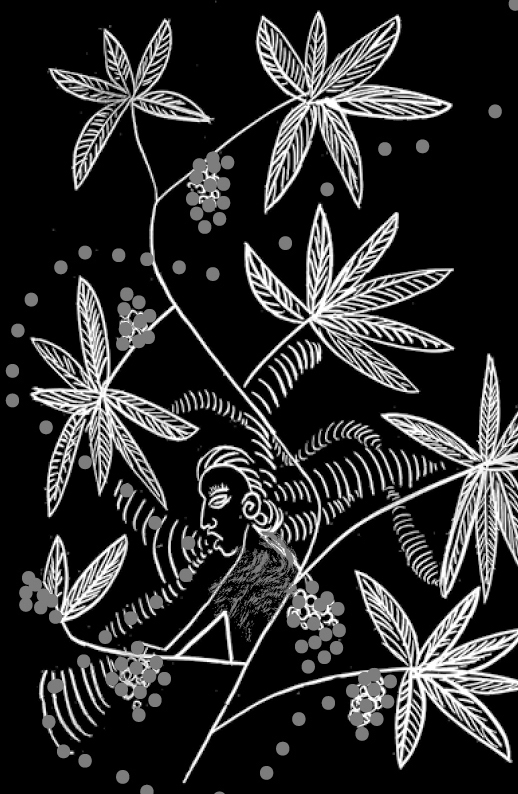
\includegraphics[width=138mm]{./imgs/img3.jpg}
\end{figure}

\chapter*{}

\mbox{}\vspace*{\fill}

O homem hup ficou
lá a noite toda e,
depois, o outro dia
inteiro. Escutou e
prendeu os cantos
do homem-sombra.

\bigskip

Hiwag yi’iy mah,
d’ú’ tɨh yam d’ö’öp\ldots{}

\vspace*{\fill}

\begin{figure}
\vspace*{-1.2cm}
\hspace*{-2.2cm}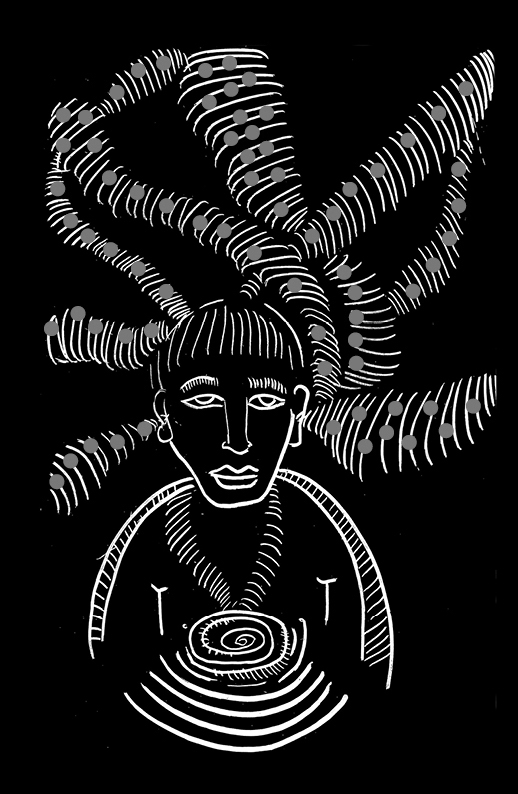
\includegraphics[width=138mm]{./imgs/img4.jpg}
\end{figure}

\chapter*{}

\mbox{}\vspace*{\fill}

Quando o sol
começou a nascer,
o homem hup bateu
com o terçado no
tronco da árvore
de cucura.

\bigskip

Hiwag yi’iy, wag
hiyèt mah tɨh kit
hik’ëtayah, tɨh
tëgët, pɨ̗g tëgët.

\vspace*{\fill}

\begin{figure}
\vspace*{-1.2cm}
\hspace*{-2.2cm}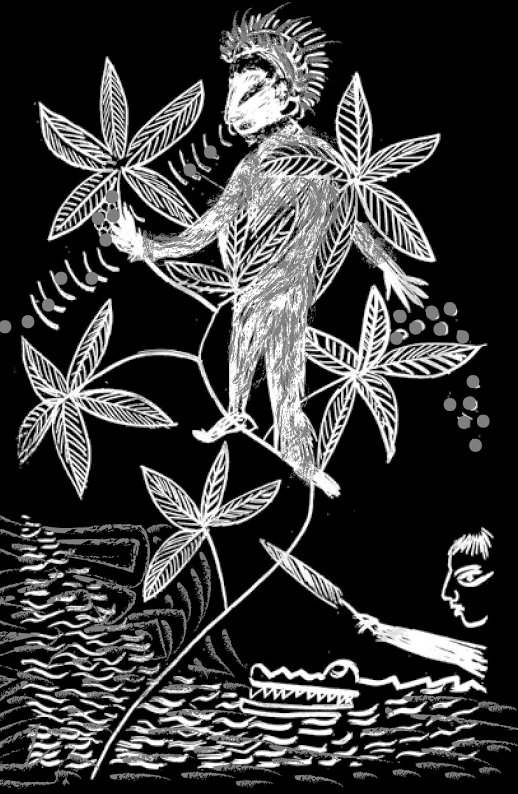
\includegraphics[width=138mm]{./imgs/img5.jpg}
\end{figure}

\chapter*{}

\mbox{}\vspace*{\fill}

Tac! Foi o barulhão
que fez. Assustado,
o Way Naku caiu da
árvore. Puffff!
Com medo, o homem
hup foi embora
correndo, bem
rápido! Vrummm!

\bigskip

Täk! nomi’, yuway
mah tɨh kädhiayah.
Pë’ ! Yuway mah
húp to’oh kädham
yi’ayah! Mmmm’ !

\vspace*{\fill}

\begin{figure}
\vspace*{-1.2cm}
\hspace*{-2.2cm}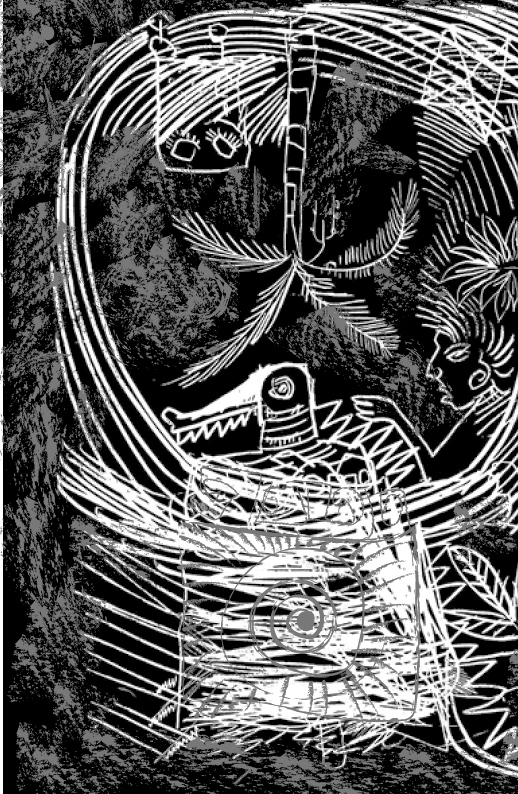
\includegraphics[width=138mm]{./imgs/img6.jpg}
\end{figure}

\chapter*{}

\mbox{}\vspace*{\fill}

Então, o Way Naku viu um
jacaré que estava deitado
na beira do rio. Pensou
que fosse o homem hup e
tentou pegá-lo. Fugindo,
o jacaré caiu na água,
tchibum! O Way Naku,
que já estava na água,
foi atrás do jacaré. O
homem-sombra colocou a
mão na água para ver se
encontrava o jacaré.


De repente, o jacaré deu
uma mordida no braço do
homem-sombra.

\bigskip

Yit mah hàt yetníh. Yit
mah hàt noh tu’uh, tapuh !
Yit mah tɨhit yi’ batɨ̗b’ noh
tu’ won kädd’öböh. Yit
mah hàtan tɨh d’ö’ yi’ih,
pëpë’ d’ö’ yi’iy.

Yit mah tɨhan tɨh k’äç
d’ö’ pög b’ayah, hàt
b’ayah, tinih mumùy súm,
batɨ̗b’anah.

\vspace*{\fill}

\begin{figure}
\vspace*{-1.2cm}
\hspace*{-2.2cm}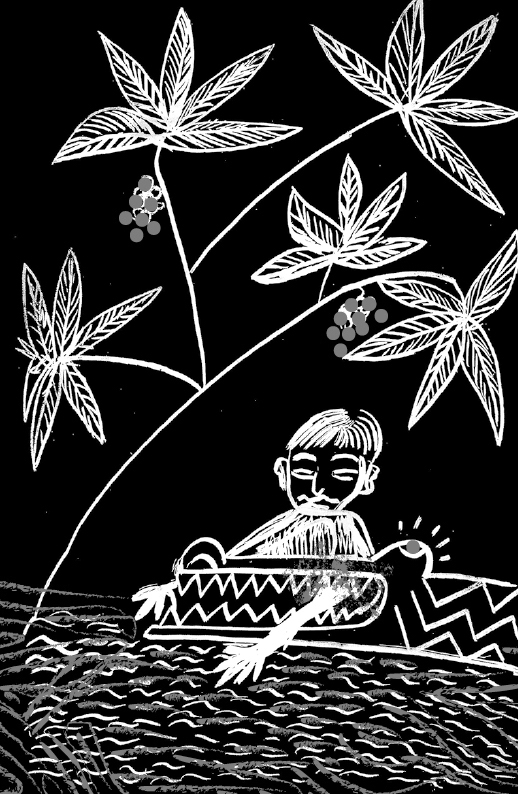
\includegraphics[width=138mm]{./imgs/img7.jpg}
\end{figure}

\chapter*{}

\mbox{}\vspace*{\fill}

E foi assim que
o homem hup
conseguiu fugir e
voltar para casa.

Esse foi o primeiro
homem hup que
soube cantar
os \textit{caapivaiá}, os
cantos das festas.

\bigskip

tɨhɨp húpup ham
yi’ay mah kah, yë
yi’ay mah.

Yup ih mah yup, yám
d’ö’ hib’ahayah.

\vspace*{\fill}

\begin{figure}
\vspace*{-1.2cm}
\hspace*{-2.2cm}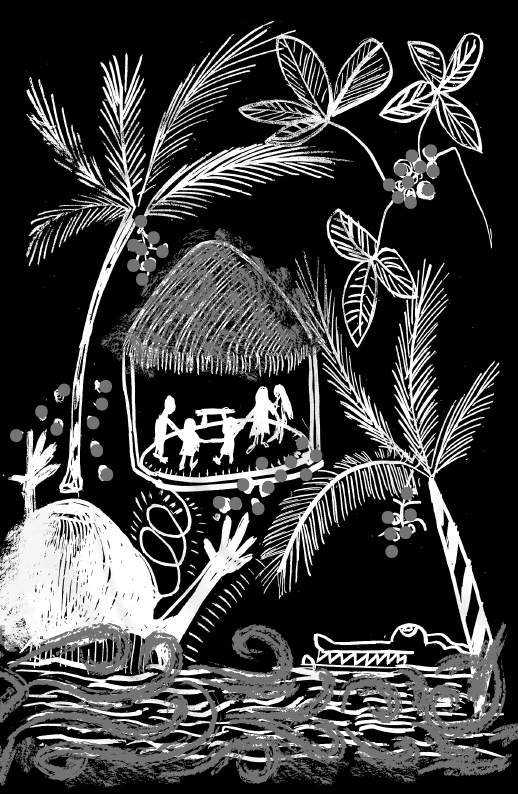
\includegraphics[width=138mm]{./imgs/img8.jpg}
\end{figure}

\chapter*{}

\mbox{}\vspace*{\fill}

Ele ouviu o homem-sombra cantar,
aprendeu bem e
começou a ensinar
para seus filhos,
irmãos, cunhados.
E até hoje todos
cantam e dançam os
caapivaiá que animam
nossas festas.

Foi isso o que ouvi de
meus avós.

\bigskip

Ya’ap meh yi’ ãh wi’ih.

Batɨ̗b’ tɨh yamawan
wi’yö’ay mah, yup húp
yamayah. Yup hid yam
tëg n’ihayah. Húpd’äh
hid yam tëgayah.

\vspace*{\fill}

\begin{figure}
\vspace*{-1.2cm}
\hspace*{-2.2cm}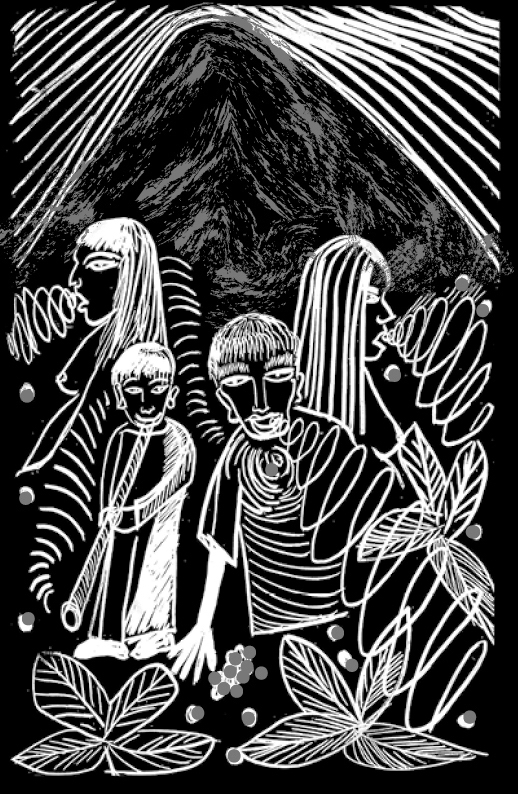
\includegraphics[width=138mm]{./imgs/img9.jpg}
\end{figure}

\chapter{Um canto do homem-sombra}

\begin{verse}
Outro galho de cucura\\
Outro galho de cucura\\
Eu jogo para baixo

Outro galho de cucura\\
Eu jogo para baixo\\
Colho o cacho de cucura\\
Eu jogo para baixo

Way Naku, yari nóóy mah\\
Marika, Way Naku
\end{verse}

\chapter{Way Naku}

\begin{verse}
Sãp nowot pɨ̗g\\
Sãp nowot pɨ̗g\\
Ãh d’äräh hitëh

Sãp nowot pɨ̗g\\
Ãh d’äräh hitëh\\
Öy d’ö’ yö’ pɨ̗g\\
Ãh d’äräh hitëh

Way Naku, yari nóóy mah\\
Marika, Way Naku
\end{verse}









